\documentclass[twoside]{article}
\usepackage[utf8]{inputenc}
\usepackage[ngerman]{babel}
\usepackage{libertine}
\usepackage[a4paper]{geometry}
\usepackage{parskip}
\usepackage{blindtext}
\usepackage{amsmath, amsthm, amssymb, commath, mathtools}
\usepackage{booktabs}
\usepackage{tabularx}
\usepackage{enumitem}
\usepackage{graphicx}
\usepackage{minted}
\usepackage{appendix}
\usepackage{icomma}

\usepackage{csquotes}
\MakeOuterQuote{"}
\renewcommand{\ttdefault}{cmtt}

\usepackage{hyperref}
\hypersetup{
	pdftitle={P1 -- STV Auswertung},
	pdfauthor={Yudong Sun, Andreas Artz},
	bookmarksnumbered=true,
	bookmarksopen=true,
	bookmarksopenlevel=2,
	pdfstartview=Fit,
	pdfpagemode=UseOutlines,
	colorlinks=true,
	linkcolor=black,
	filecolor=magenta,      
	urlcolor=blue
}
\urlstyle{same}

\title{STV -- Statistische Verteilung \\ Auswertung}
\author{Yudong Sun, Andreas Artz \\ Gruppe F2}

\newcommand{\versuch}[0]{STV}

\usepackage{fancyhdr}
 
\pagestyle{fancy}
\fancyhf{}
\fancyhead[RO]{Yudong Sun, Andreas Artz}
\fancyhead[LO]{Auswertung -- \versuch}
\fancyhead[LE]{Yudong Sun, Andreas Artz}
\fancyhead[RE]{Auswertung -- \versuch}
\cfoot{\thepage}

\begin{document}

\maketitle

\section*{Teilversuch 1: Generierung einer Binomialverteilung mit dem Galton-Brett}

    \subsection*{Annahme: Die Verteilung der Kugeln ist bekannt}
        Bei jeder Weggabelung kann die Kugel entweder links oder rechts fallen. Damit die Kugel in den 0. Kanal fällt muss sie bei jeder Weggabelung im Galton-Brett nach links fallen, also insgesamt 10 mal. 
        \begin{align*}
            p(\text{Eine Kugel in Kanal 0}) &=\binom{10}{10} \times \frac{1}{2}^{10} \times \frac{1}{2}^0 \\
            &= \frac{1}{2^{10}} = 0.097\% 
        \end{align*}
        Damit die Kugel in den 5. Kanal, der genau in der Mitte liegt, fällt, muss sie bei den Weggabelungen insgesamt 5 mal nach links und 5 mal nach rechts fallen. Die Reihenfolge ist dabei egal.
        \begin{align*}
            p(\text{Eine Kugel in Kanal 5}) &=\binom{10}{5} \times \frac{1}{2}^{5} \times \frac{1}{2}^{5} \\
            &= 24.6\% 
        \end{align*}
        
    \pagebreak
    \subsection*{Annahme: Die Verteilung der Kugeln ist unbekannt}
    
        \begin{figure}[!ht]
            \centering
            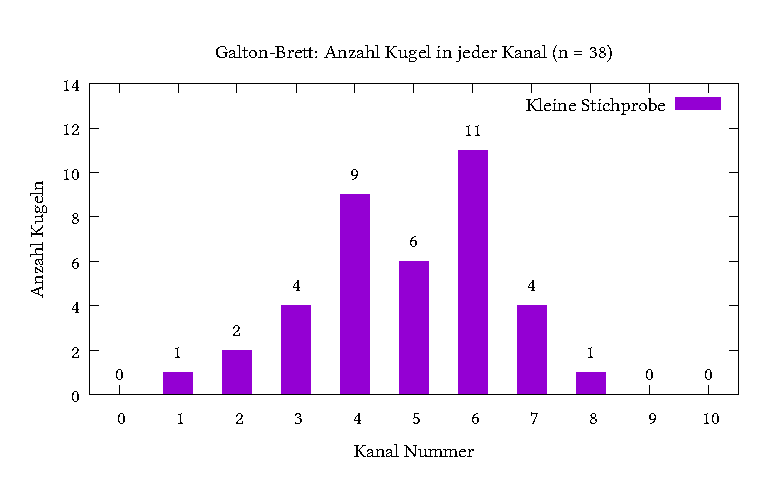
\includegraphics{kleine.eps}
            \caption{Histogramm der kleinen Statistik}
            \label{fig:kleine_histo}
        \end{figure}
        
        Die Mittelwert und Standardabweichung wird mithilfe eines Python-Skripts berechnet (Siehe Appendix \ref{appdx:codes}):
         \begin{center}
            \begin{tabular}{l l}
                \toprule
                Mittelwert & $4,8684$ \\
                Standardabweichung & $1,5968$ \\
                \bottomrule
            \end{tabular}
        \end{center}
        
         Man kann vom Histogramm nicht auf eine Binomialverteilung schließen. Zumindest ist das Histogramm nicht symmetrisch, und das Maximum ist nicht beim Mittelwert.
        
    \subsection*{Diskussion}
        Die Häufigkeits\-verteilungen sollten sich mit wachsender Stichprobengröße der Wahrscheinlichkeitsfunktion der Binomial\-verteilung annähern. Das Ergebnis zeigt dies, da die Verteilung der großen Statistik deutlich symmetrischer ist als die der mittleren Statistik. Zudem ist der Mittelwert der großen Statistik näher am Erwartungswert.
        
        Der Fehler wird so berechnet: $\lvert E(x) - \bar{x} \rvert$

        \begin{center}
            \begin{tabular}{l | l l l}
                \toprule
                Stichprobe & Mittelwert & Standardabweichung & Fehler \\
                \midrule
                Klein & $4,868$ & $1,5968$ & $0,134$ \\
                Mittel & $4,832$ & $1,6327$ & $0,168$ \\
                Groß & $4,915$ & $1,6237$ & $0,085$ \\
                \bottomrule
            \end{tabular}
        \end{center}

\pagebreak
\section*{Teilversuch 3: Zentrale Grenzwertsatz}
    Die Standardabweichung aus Teilversuch 2 wird mit dem vorgenannten Python Skript berechnet.\footnote{Mit dieser neuen Berechnung ist das Problem beim Ablesen im MATLAB während des Versuchs auch bekannt gemacht: Die Dateien sind im \texttt{UTF-16LE} und nicht \texttt{UTF-8} codiert.} Für 100 Messungen je 2 Sekunden haben wir das folgende Ergebnis:
    
    \begin{center}
            \begin{tabular}{l | l l l}
                \toprule
                Teilversuch & Mittelwert & Standardabweichung & Varianz \\
                \midrule
                2 & $2,36$ & $1,3681$ & $1,872$ \\
                3 & $77,54$ & $8,9594$ & $80.271$ \\
                \bottomrule
            \end{tabular}
        \end{center}

    \subsection*{Variante 1}
        Diese Variante wurde wegen zeitlicher Gründe nicht untersucht.
    \subsection*{Variante 2}
        Der zentrale Grenzwertsatz besagt, dass die Verteilung jeder beliebig verteilten Zufallsvariable in einer Stichprobe aus $n$ unabhängigen Messungen sich mit wachsendem $n$ einer Normalverteilung annähern wird. 
        
        In diesem Fall, wird das ROI bzw. Energieintervall im Vergleich zu vorher vergrößert. Die Zufallsvariable in diesem Fall ist die Anzahl der Impulse je 2 Sekunden. Wenn man diese Anzahl von alle Kanäle summiert, hat man nun durchschnittlich $77,54$ Impulse pro Zeiteinheit, statt durchschnittlich nur $2,36$ Impulse pro Zeiteinheit im Teilversuch 2. Das entspricht die Situation, indem man ein Poisson-verteilte Variable mehrmals messen, sodass man laut ZGS eine Normalverteilung bekommen. 
        
\appendix
\newpage
\section{Quellcode zur Auswertung von Teilversuch 1}
    \label{appdx:codes}
    
    \texttt{gnuplot} Code für Abbildung \ref{fig:kleine_histo}
    \begin{minted}[linenos,breaklines,autogobble,frame=leftline,framesep=10pt]{gnuplot}
        set term epscairo font 'Linux Libertine, 14'
        set output "kleine.eps"
        
        set xrange [-0.5:10.5]
        set yrange [0:14]
        set xtics 1
        set title "Galton-Brett: Anzahl Kugel in jeder Kanal (n = 38)"
        set ylabel "Anzahl Kugeln"
        set xlabel "Kanal Nummer"
        
        set boxwidth 0.5
        set style fill solid
        plot "kleine.dat" w boxes title "Kleine Stichprobe", "" u 1:2:2 with labels offset char 0,1 notitle
    \end{minted}
    
    \texttt{Python} Code für die Rechnung der Mittelwert und Standardabweichung:
    \begin{minted}[linenos,breaklines,autogobble,frame=leftline,framesep=10pt]{python}
        #!/usr/bin/env python3

        import numpy as np
        
        with open("kleine.dat") as f:
        	A = np.loadtxt(f, dtype=int)
        	kanale = A[:,0] # Erste Spalte
        	anzahl = A[:,1] # Zweite Spalte
        
        # Mittelwert
        mit = np.dot(kanale, anzahl)/np.sum(anzahl)
        
        # Standardabweichung
        sab = np.sqrt((1/(np.sum(anzahl) - 1))*np.dot((kanale - mit)**2, anzahl))
        
        print("Mittelwert: ", mit)
        print("Standardabweichung: ", sab)
    \end{minted}

    \texttt{kleine.dat};
    \begin{minted}[linenos,breaklines,autogobble,frame=leftline,framesep=10pt]{text}
        0    0
        1    1
        2    2
        3    4
        4    9
        5    6
        6    11
        7    4
        8    1
        9    0
        10   0
    \end{minted}


\end{document}
